\chapter{What Counts as a Law of Motion?}

Classical mechanics begins, in this lecture, with a question that is broader than any one planetary orbit or any one falling body. We want to know not only the specific laws for particular systems, but also the general shape that an allowable law of motion must have. Leonard Susskind opens with deliberately tiny worlds in order to make that question visible before physics becomes cluttered with detail. The present notes follow that order closely, and the preserved board frames from LazyingArt LLC and Video2Book are used only where they steady an equation or a diagram already motivated in the lecture itself.

\section{Two Questions and a Minimal World}

There are, from the outset, two different kinds of question. One may ask for the law governing a particular system: a planet near a heavy mass, or a charged particle in a magnetic field. But one may also ask a more structural question: what are the rules that an acceptable law of motion must satisfy at all?

It is this second question that governs the lecture. The specific examples are not digressions. They are stripped-down laboratories in which the notions of state, law, determinism, conservation, and reversibility can be seen without distraction.

So we begin with the smallest nontrivial world Susskind can imagine: a coin lying on an abstract table. The coin has only two configurations,
\[
H \qquad \text{and} \qquad T,
\]
and nothing else about it matters. An initial condition is just the choice of one of these two states at the initial time. A law of motion is then an update rule telling us what the next state will be.

This order is important. First we decide what the states are. Only afterward do we ask how they evolve.

\section{A Coin as a Dynamical System}

The coin has two possible configurations,
\[
\mathcal{C}=\{H,T\}.
\]
At first we imagine time as stroboscopic and discrete. We look only at successive flashes, and so the time variable takes integer values,
\[
t\in \mathbb{Z}.
\]

\paragraph{The trivial law.}
The most boring law is also the first clean example of determinism:
\[
H\to H,\qquad T\to T.
\]
Nothing happens. But precisely because nothing happens, the future is completely fixed once the initial condition is given. If we begin with heads, the entire history is
\[
H,H,H,H,\dots
\]
and if we begin with tails, it is
\[
T,T,T,T,\dots
\]

\paragraph{The flip law.}
There is only one other deterministic one-step law for a two-state system:
\[
H\to T,\qquad T\to H.
\]
This is the first genuinely dynamical example.

\begin{figure}
\centering

\includegraphics[width=0.78\textwidth]{lecture_01_figure_02.png}
\caption{Board layout for the two-state heads-tails update rule. The screenshot is kept as documentary evidence of the lecture board.}
\end{figure}

\begin{figure}
\centering
\begin{tikzpicture}[scale=1.0]
\draw (0,0) rectangle (2.2,1.3);
\node at (1.1,0.65) {$H,\ T$};

\draw (4.4,0.0) circle (0.45);
\draw (6.4,0.0) circle (0.45);
\node at (4.4,0.0) {$H$};
\node at (6.4,0.0) {$T$};

\draw[->] (4.72,0.28) .. controls (5.35,1.15) and (5.45,1.15) .. (6.08,0.28);
\draw[->] (6.08,-0.28) .. controls (5.45,-1.15) and (5.35,-1.15) .. (4.72,-0.28);

\node at (5.4,-1.8) {$H\to T,\qquad T\to H$};
\end{tikzpicture}
\caption{Clean reconstruction of the two-state flip law.}
\end{figure}

Only after the picture is clear does Susskind introduce notation. We let
\[
\sigma=
\begin{cases}
1,& \text{for } H,\\[4pt]
-1,& \text{for } T.
\end{cases}
\]
Then the two configurations are represented by the two values of a single variable.

The trivial law becomes
\begin{equation}
\sigma(t+1)=\sigma(t),
\end{equation}
while the flip law becomes
\begin{equation}
\sigma(t+1)=-\sigma(t).
\end{equation}

\begin{figure}
\centering

\includegraphics[width=0.78\textwidth]{lecture_01_figure_03.png}
\caption{The same two-state system after the lecture upgrades it to sigma notation.}
\end{figure}

\begin{figure}
\centering
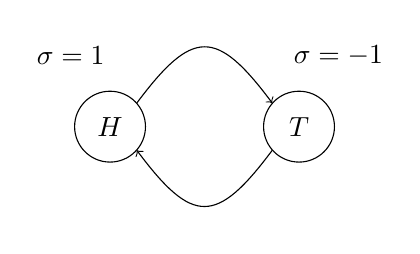
\begin{tikzpicture}[scale=1.0]
\draw (3.8,0.0) circle (0.45);
\draw (6.2,0.0) circle (0.45);
\node at (3.8,0.0) {$H$};
\node at (6.2,0.0) {$T$};
\node at (3.3,0.9) {$\sigma=1$};
\node at (6.7,0.9) {$\sigma=-1$};

\draw[->] (4.14,0.30) .. controls (4.85,1.25) and (5.15,1.25) .. (5.86,0.30);
\draw[->] (5.86,-0.30) .. controls (5.15,-1.25) and (4.85,-1.25) .. (4.14,-0.30);
\end{tikzpicture}
\caption{Clean reconstruction of the sigma-labeled coin system.}
\end{figure}

The point of the example is not the coin. The point is that once the system is closed and the law is specified, the future is determined. Classical mechanics, at least in the framework being laid out here, is deterministic for closed systems.

\section{From a Coin to a Die: Cycles, Relabeling, and Conservation}

We now enlarge the state space but keep the logic exactly the same. A die has six states,
\[
1,2,3,4,5,6,
\]
and an initial condition is again just the choice of one of these states at the initial time.

For the die, Susskind prefers not to write an explicit equation immediately. The graph is more illuminating. A law of motion is represented by arrows, and the history of the system is obtained by following them.

A simple nontrivial law is the six-cycle
\begin{equation}
1\to 2\to 3\to 4\to 5\to 6\to 1.
\end{equation}
The exact spoken line in the lecture is slightly garbled at one point, but the intended cycle is clear from the context and from the histories he describes.

\begin{figure}
\centering
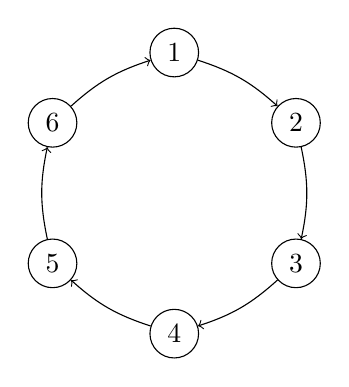
\begin{tikzpicture}[scale=1.05]
\node[circle,draw] (1) at (90:1.7) {$1$};
\node[circle,draw] (2) at (30:1.7) {$2$};
\node[circle,draw] (3) at (-30:1.7) {$3$};
\node[circle,draw] (4) at (-90:1.7) {$4$};
\node[circle,draw] (5) at (-150:1.7) {$5$};
\node[circle,draw] (6) at (150:1.7) {$6$};

\draw[->] (1) to[bend left=12] (2);
\draw[->] (2) to[bend left=12] (3);
\draw[->] (3) to[bend left=12] (4);
\draw[->] (4) to[bend left=12] (5);
\draw[->] (5) to[bend left=12] (6);
\draw[->] (6) to[bend left=12] (1);
\end{tikzpicture}
\caption{A single six-cycle. Different drawings with the same single-cycle structure are merely relabelings of one another.}
\end{figure}

Now we can write another law,
\[
1\to 2,\qquad 2\to 5,\qquad 5\to 3,\qquad 3\to 4,\qquad 4\to 6,\qquad 6\to 1,
\]
but this is not genuinely new. It is still one cycle passing through all six states. It differs only by a relabeling.

A genuinely different law is one with disconnected cycles. For example, we may have
\[
1\to 2\to 3\to 1
\]
and separately
\[
4\to 6\to 5\to 4.
\]
Then if the system starts on one cycle, it never reaches the other.

\begin{figure}
\centering
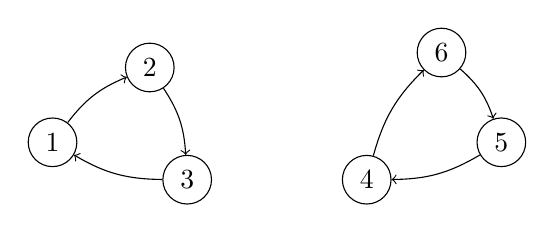
\begin{tikzpicture}[scale=0.95]
\node[circle,draw] (1) at (-3.0,1.0) {$1$};
\node[circle,draw] (2) at (-1.7,2.0) {$2$};
\node[circle,draw] (3) at (-1.2,0.5) {$3$};

\node[circle,draw] (4) at (1.2,0.5) {$4$};
\node[circle,draw] (5) at (3.0,1.0) {$5$};
\node[circle,draw] (6) at (2.2,2.2) {$6$};

\draw[->] (1) to[bend left=15] (2);
\draw[->] (2) to[bend left=15] (3);
\draw[->] (3) to[bend left=15] (1);

\draw[->] (4) to[bend left=15] (6);
\draw[->] (6) to[bend left=15] (5);
\draw[->] (5) to[bend left=15] (4);
\end{tikzpicture}
\caption{A law with two disconnected cycles. The disconnected pieces carry a conserved label.}
\end{figure}

This brings in the first real notion of conservation. We may assign one label to the upper cycle and another to the lower. That label does not change with time. The state changes, but the cycle-label does not.

\begin{definition}
A conserved quantity is a label on the state space that remains constant under the evolution.
\end{definition}

In these toy examples, conserved quantities arise because state space decomposes into disconnected cycles.

\subsection{Question \& Answer}

\paragraph{Question.} What if the next step depends not only on the present configuration, but also on the previous one?

\paragraph{Answer.} Then the present configuration alone was never the true state. The state must be enlarged until one-step prediction becomes possible.

For the coin, if the next value depends on both the current and the previous configuration, then the relevant state space is not merely \(\{H,T\}\). It is the four-element set
\[
\{HH,HT,TH,TT\},
\]
where, for example, \(HT\) means ``heads now, tails one step ago.''

This is the crucial sharpening of language:

\begin{definition}
The state of a system consists of all the data that must be known at one time in order to predict the future.
\end{definition}

What began as a childish example has now produced a serious principle. We do not get to decide arbitrarily what the state is. The dynamics decides it for us.

\section{Infinite State Spaces and the Meaning of an Allowed Law}

The same ideas survive intact when the number of states becomes infinite. Consider a particle that can occupy any integer point on an infinite line. We label its position by an integer \(n\in\mathbb{Z}\).

One possible law is
\begin{equation}
n(t+1)=n(t)+1.
\end{equation}
At each step the particle moves one unit to the right. There is only one endless orbit: if we follow the arrows far enough, we pass through every integer.

Another law is
\begin{equation}
n(t+1)=n(t)+2.
\end{equation}
Now the even integers talk only to the even integers, and the odd integers talk only to the odd integers. The conserved quantity is parity.

\begin{figure}
\centering
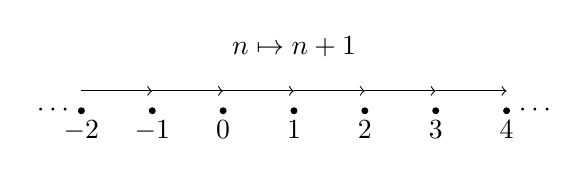
\begin{tikzpicture}[scale=0.9]
\foreach \x/\lab in {0/{-2},1/{-1},2/{0},3/{1},4/{2},5/{3},6/{4}}{
  \fill (\x,0) circle (1.4pt);
  \node[below] at (\x,0) {$\lab$};
}
\foreach \x in {0,1,2,3,4,5}{
  \draw[->] (\x,0.28) -- (\x+1,0.28);
}
\node at (3,0.9) {$n\mapsto n+1$};
\node at (-0.4,0) {$\cdots$};
\node at (6.4,0) {$\cdots$};
\end{tikzpicture}

\vspace{0.8cm}

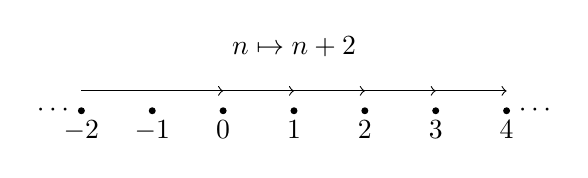
\begin{tikzpicture}[scale=0.9]
\foreach \x/\lab in {0/{-2},1/{-1},2/{0},3/{1},4/{2},5/{3},6/{4}}{
  \fill (\x,0) circle (1.4pt);
  \node[below] at (\x,0) {$\lab$};
}
\foreach \x in {0,1,2,3,4}{
  \draw[->] (\x,0.28) -- (\x+2,0.28);
}
\node at (3,0.9) {$n\mapsto n+2$};
\node at (-0.4,0) {$\cdots$};
\node at (6.4,0) {$\cdots$};
\end{tikzpicture}
\caption{Two infinite-state laws on the integer lattice. The second preserves parity.}
\end{figure}

A convenient encoding is
\[
Q_{\mathrm{parity}}(n)=
\begin{cases}
0,& n \text{ even},\\[4pt]
1,& n \text{ odd}.
\end{cases}
\]
Under the rule \(n\mapsto n+2\), this quantity is conserved.

So far, however, every law we have written has shared a deeper property. It predicts the future, and it also lets us reconstruct the past. Susskind now introduces a law that breaks this second feature.

Take a three-state system with states \(H\), \(T\), and \(E\) (for ``edge''). Let the update rule be
\[
H\to T,\qquad T\to E,\qquad E\to T.
\]
This predicts the future perfectly. But it does not predict the past: if we are at \(T\), we do not know whether we came from \(H\) or from \(E\).

\begin{figure}
\centering
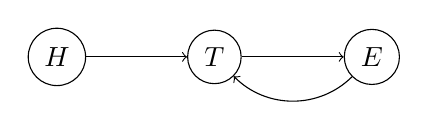
\begin{tikzpicture}[scale=1.0]
\node[circle,draw] (H) at (-2,0) {$H$};
\node[circle,draw] (T) at (0,0) {$T$};
\node[circle,draw] (E) at (2,0) {$E$};

\draw[->] (H) -- (T);
\draw[->] (T) -- (E);
\draw[->] (E) to[bend left=45] (T);
\end{tikzpicture}
\caption{A future-deterministic law that is not reversible. Two different states feed into \(T\).}
\end{figure}

\subsection{Question \& Answer}

\paragraph{Question.} Why is this law not allowed, if it still predicts the future?

\paragraph{Answer.} Because classical mechanics demands more than forward predictability. It demands reversibility.

If we reverse every arrow in the three-state graph, the reversed graph is no longer predictive: from \(T\) there are now two possible next moves. Thus the original law can be run forward but not backward.

\begin{definition}
A law is reversible if the present state determines both the next state and the previous state. In the graph language, this means that each state has exactly one outgoing arrow and exactly one incoming arrow.
\end{definition}

This is the central structural claim of the first half of the lecture. A legal classical law is not merely deterministic into the future. It is deterministic into the past as well.

\section{Exact Laws, Imperfect Initial Data, and the Pivot to Particles}

At this point one might be tempted to conclude that classical mechanics gives unlimited predictive power. Susskind immediately qualifies that claim.

To predict the future we need two things:
\begin{itemize}
\item the law of motion,
\item the initial condition.
\end{itemize}
Even when the law is exact, our knowledge of the initial condition may not be.

In the discrete toy systems it is easy to imagine perfect knowledge. One can simply look at the coin. But the real world is not like that. The positions and velocities of particles are continuous quantities. No matter how many decimal places are measured, they are never known exactly.

Thus there is an unavoidable distinction between exact law and practical prediction. Some systems amplify small errors violently. The weather is Susskind's example. If the atmospheric state is known only approximately, then the uncertainty in the forecast grows, and after long enough the future becomes unpredictable in practice even though the equations remain perfectly definite.

This is not a retreat from determinism. It is a reminder that determinism belongs to the law, whereas prediction also depends on knowledge.

From here the lecture turns to the more realistic world of particles. But before we can write their laws, we need a mathematical language for configuration space in the continuous setting. That language is the language of coordinates and vectors.

\section{Coordinates, Vectors, and the Algebra We Need}

We now pass from finite state spaces to ordinary space. For the moment, space is taken to be three-dimensional. A point is described by Cartesian coordinates
\[
(x,y,z),
\]
or, equivalently,
\[
(x_1,x_2,x_3).
\]

We choose:
\begin{itemize}
\item an origin,
\item three mutually perpendicular axes,
\item an orientation,
\item units of length.
\end{itemize}
Once the \(x\)- and \(y\)-directions are fixed, there remains one discrete choice for the direction of the \(z\)-axis. The lecture adopts the standard right-handed convention.

\begin{figure}
\centering
\begin{tikzpicture}[scale=1.15]
\draw[->] (0,0) -- (2.5,0) node[right] {$x$};
\draw[->] (0,0) -- (0,2.4) node[above] {$y$};
\draw[->] (0,0) -- (-1.3,-0.9) node[below] {$z$};

\fill (1.6,1.35) circle (1.2pt);
\draw[->] (0,0) -- (1.6,1.35) node[midway, above left] {$\vec r$};
\draw[dashed] (1.6,1.35) -- (1.6,0);
\draw[dashed] (1.6,1.35) -- (0,1.35);
\node[below] at (1.6,0) {$x$};
\node[left] at (0,1.35) {$y$};
\end{tikzpicture}
\caption{A point in a right-handed Cartesian coordinate system, together with its position vector.}
\end{figure}

A vector is an object with magnitude and direction. It is not, in the first instance, tied to a specific location in space. We may redraw it elsewhere without changing the vector itself.

If a vector has components \((v_x,v_y,v_z)\), its magnitude is
\begin{equation}
|\vec v|=\sqrt{v_x^2+v_y^2+v_z^2}.
\end{equation}
This is just Pythagoras in three dimensions.

Vectors may be multiplied by ordinary numbers. If \(c>0\), the vector \(c\vec A\) points in the same direction as \(\vec A\) but has magnitude \(c|\vec A|\). If \(c<0\), the direction is reversed.

Vectors may also be added. Geometrically, we may place the tail of \(\vec B\) at the head of \(\vec A\), and the third side of the resulting triangle is \(\vec A+\vec B\). In components,
\begin{equation}
C_i=A_i+B_i.
\end{equation}

The most important vector product for the lecture is the dot product. If \(\theta\) is the angle between \(\vec A\) and \(\vec B\), then
\begin{equation}
\vec A\cdot \vec B = |\vec A|\,|\vec B|\cos\theta.
\end{equation}
The same quantity can also be written in components as
\begin{equation}
\vec A\cdot \vec B=A_xB_x+A_yB_y+A_zB_z.
\end{equation}
In particular,
\begin{equation}
\vec A\cdot \vec A=|\vec A|^2.
\end{equation}
This gives a clean diagnostic for orthogonality: two vectors are perpendicular exactly when their dot product vanishes.

\begin{figure}
\centering

\includegraphics[width=0.70\textwidth]{lecture_01_figure_04.png}
\caption{Board derivation of the law of cosines from vector subtraction. The lecture board mixes bars and arrows; the notes normalize to arrow notation.}
\end{figure}

The lecture then uses this machinery to derive the law of cosines. There is a small but instructive live correction on the board: Susskind first says \(\vec C=\vec A+\vec B\), then corrects himself. For the side drawn in the sketch one needs
\[
\vec C=\vec A-\vec B.
\]
Now compute:
\begin{align}
|\vec C|^2
  &= \vec C\cdot\vec C \\
  &= (\vec A-\vec B)\cdot(\vec A-\vec B) \\
  &= \vec A\cdot\vec A+\vec B\cdot\vec B-2\vec A\cdot\vec B \\
  &= |\vec A|^2+|\vec B|^2-2|\vec A|\,|\vec B|\cos\theta.
\end{align}
This is the law of cosines in vector form.

\begin{figure}
\centering
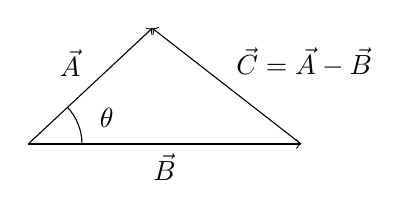
\begin{tikzpicture}[scale=1.05]
\coordinate (O) at (0,0);
\coordinate (A) at (1.5,1.4);
\coordinate (B) at (3.3,0);

\draw[->] (O) -- (A) node[midway, above left] {$\vec A$};
\draw[->] (O) -- (B) node[midway, below] {$\vec B$};
\draw[->] (B) -- (A) node[midway, above right] {$\vec C=\vec A-\vec B$};

\draw (0.65,0) arc (0:43:0.65);
\node at (0.95,0.32) {$\theta$};
\end{tikzpicture}
\caption{Clean reconstruction of the vector-subtraction triangle used in the law-of-cosines derivation.}
\end{figure}

By the end of this section we have the minimal algebra needed to begin mechanics proper.

\section{Position, Velocity, Acceleration, and Two Motion Examples}

A point particle at time \(t\) is described by its position vector
\[
\vec r(t)=(x(t),y(t),z(t)).
\]
Its components are just the coordinates of the particle.

The velocity is the time derivative of position. In components,
\begin{equation}
v_i=\frac{dx_i}{dt}=\dot x_i,
\end{equation}
and in vector form,
\begin{equation}
\vec v=\frac{d\vec r}{dt}=\dot{\vec r}.
\end{equation}
Likewise, acceleration is the time derivative of velocity,
\begin{equation}
a_i=\dot v_i=\ddot x_i,
\qquad
\vec a=\frac{d\vec v}{dt}=\frac{d^2\vec r}{dt^2}=\ddot{\vec r}.
\end{equation}

\begin{figure}
\centering

\includegraphics[width=0.78\textwidth]{lecture_01_figure_05.png}
\caption{The lecture board moving from component notation to the vector statement \(\vec v=d\vec r/dt\).}
\end{figure}

The board at this point uses uppercase \(V_i\) and \(X_i\), but the lecture itself does not insist on that choice. We normalize here to lower-case component notation.

\paragraph{First example: motion along a line.}
If the particle moves only along the \(x\)-axis, then one may write
\begin{equation}
x(t)=a+bt+ct^2.
\end{equation}
The velocity is
\begin{equation}
\dot x(t)=b+2ct,
\end{equation}
and the acceleration is
\begin{equation}
\ddot x(t)=2c.
\end{equation}
Thus the acceleration is constant. At \(t=0\) the particle is at \(x=a\), and its initial velocity is \(b\). This is the simplest example of uniformly accelerated motion.

\paragraph{Second example: uniform circular motion.}
Now let a particle move on the unit circle in the \(xy\)-plane. The angular position is taken to increase linearly with time,
\begin{equation}
\theta(t)=\omega t.
\end{equation}
One full revolution corresponds to \(\theta=2\pi\), so the period is
\begin{equation}
T=\frac{2\pi}{\omega}.
\end{equation}
Since the radius is one, the position components are
\begin{equation}
x(t)=\cos(\omega t),\qquad y(t)=\sin(\omega t).
\end{equation}

\begin{figure}
\centering
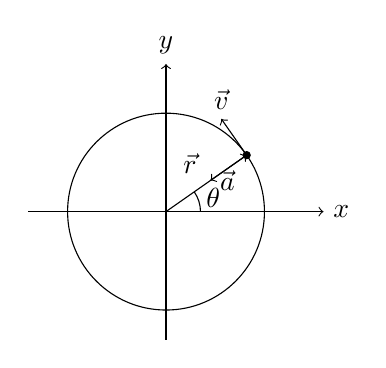
\begin{tikzpicture}[scale=1.25]
\draw[->] (-1.4,0) -- (1.6,0) node[right] {$x$};
\draw[->] (0,-1.3) -- (0,1.5) node[above] {$y$};
\draw (0,0) circle (1);

\coordinate (P) at ({cos(35)},{sin(35)});
\fill (P) circle (1.2pt);

\draw[->] (0,0) -- (P) node[midway, above left] {$\vec r$};
\draw[->] (P) -- ++({-0.45*sin(35)},{0.45*cos(35)}) node[above] {$\vec v$};
\draw[->] (P) -- ++({-0.45*cos(35)},{-0.45*sin(35)}) node[right] {$\vec a$};

\draw (0.35,0) arc (0:35:0.35);
\node at (0.48,0.14) {$\theta$};
\end{tikzpicture}
\caption{Uniform circular motion on the unit circle. The velocity is tangent to the orbit, while the acceleration points inward.}
\end{figure}

Differentiating once gives the velocity components:
\begin{equation}
v_x(t)=-\omega\sin(\omega t),\qquad v_y(t)=\omega\cos(\omega t).
\end{equation}

\subsection{Question \& Answer}

\paragraph{Question.} It is geometrically obvious that the velocity should be perpendicular to the position vector. How do we prove it?

\paragraph{Answer.} Compute the dot product:
\begin{align}
\vec r\cdot\vec v
  &= x v_x + y v_y \\
  &= \cos(\omega t)\bigl(-\omega\sin(\omega t)\bigr)
   + \sin(\omega t)\bigl(\omega\cos(\omega t)\bigr) \\
  &= 0.
\end{align}
Since the dot product vanishes, \(\vec r\) and \(\vec v\) are perpendicular.

This is exactly the rhythm of the lecture: we see the geometry first, but then we insist on checking it by calculation.

Differentiate once more to obtain the acceleration:
\begin{equation}
a_x(t)=-\omega^2\cos(\omega t),\qquad a_y(t)=-\omega^2\sin(\omega t).
\end{equation}
Therefore
\begin{equation}
\vec a=-\omega^2\vec r.
\end{equation}
The acceleration is parallel to the position vector but points in the opposite direction. So it is directed inward, toward the origin. The sign matters here: the mathematics gives centripetal, not outward, acceleration.

Finally, the magnitudes are easy to compute:
\begin{align}
|\vec v|^2
  &= v_x^2+v_y^2 \\
  &= \omega^2\sin^2(\omega t)+\omega^2\cos^2(\omega t) \\
  &= \omega^2,
\end{align}
so
\[
|\vec v|=\omega.
\]
Likewise,
\begin{align}
|\vec a|^2
  &= a_x^2+a_y^2 \\
  &= \omega^4\cos^2(\omega t)+\omega^4\sin^2(\omega t) \\
  &= \omega^4,
\end{align}
and therefore
\[
|\vec a|=\omega^2.
\]

The closing examples do exactly what they were supposed to do. They turn the vector language back into mechanics.

\section{Summary}

The lecture begins far away from ordinary particle mechanics and yet arrives exactly where mechanics needs to begin. By studying coins, dice, and integer lattices, we learn what a state is, what a law is, what determinism means, how conserved quantities arise, and why classical laws must be reversible. The toy examples are not expendable. They carry the conceptual thesis.

Only then do we move to particles in space. There we introduce coordinates, vectors, the dot product, and the law of cosines, and then immediately use them to define position, velocity, and acceleration. The final payoff is modest but exact: motion on a line and motion on a circle. In the next lecture the same framework will be used to ask the real dynamical question for particles: what is the space of initial conditions, and what laws move the system from one instant to the next?